\chapter{Research Investigation}\label{chap:research-investigation}  % other option are Experimental Results, Research Exploration, Research Assessment

In this chapter we describe the research aspect of the thesis.  % TODO: add description 

\section{Research Questions}

To investigate the nature of in-context learning capabilities of Code LLMs, we consider the following research questions:

\begin{sloppypar}
\begin{description}
    \item[RQ.A1]\phantomsection\label{rq:rq-a1} \textbf{\nameref{sec:composition-impact-on-inference}:} Does the quality improvement of code completion depend on the composition strategy employed during model inference?
    \item[RQ.A2]\phantomsection\label{rq:rq-a2} \textbf{\nameref{sec:fine-tuning-on-compositions}:} Does fine-tuning a pre-trained Code LLM with a specific context composer enhance the subsequent quality of code completion?
    \item[RQ.B1]\phantomsection\label{rq:rq-b1} \textbf{\nameref{sec:effect-of-context-extension}:} Does the repository-level pre-training step affect the in-context learning abilities of the model developed during earlier stages?
    \item[RQ.B2]\phantomsection\label{rq:rq-b2} \textbf{\nameref{sec:influence-of-composition-on-context-extension}:} Does the quality improvement of code completion depend on the context composition approach used during the repository-level pre-training step?
\end{description}
\end{sloppypar}

\section{Experimental Design}

In this section, we describe the unified experimental design for all four research questions, including the data, training, and evaluation components. Specific details are deferred to the subsequent sections dedicated to each research question separately.

\subsection{Training Data}
% TODO: draw the diagram
% TODO: supporting company -> company that initialized this research
% TODO: mention JetBrains somewhere

The dataset utilized in this research was provided by the supporting company and is based on the methodology outlined in \citet{bogomolov2024}. The dataset was constructed by traversing the GitHub histories of Python repositories and applying permissive license filtering to sample completion files and their corresponding parent commits. Each data point consists of a pair: a list of Python completion files and a repository snapshot that captures the state of the repository at the time the completion files were added. The snapshot includes all text files except for the completion files themselves. To prevent contamination of the benchmark used in the evaluation, any repositories present in the benchmark were excluded from the training data.

To delineate the scope of this work, we ought to note that the corpus described thus far was entirely provided by the company and was not generated by the author of this thesis. Conversely, the subsequent processing steps applied to this dataset represent the original contributions of the author.

The multiple filtering criteria are applied to obtain the dataset with greater relevance and quality. First, all commits made prior to 2010 are excluded. Second, completion files with lengths outside the closed interval [800, 25000] characters are removed. Third, to eliminate redundancy, a simple deduplication strategy is employed on completion files based on the file name and the name of the repository to which they belong. Finally, up to 1000 of the most recently updated unique completion files are selected from each repository. The remaining repository snapshot is retained without additional processing. \parencite{sapronov2025}

The resulting corpus comprises 1,640 repositories, 160,801 commits, and 361,052 completion files. The completion files contain a total of 1.7 billion characters, while the repository snapshot files contain 4.8 trillion characters.

A subset of 2560 samples is randomly selected to form the validation set. During this process, we ensure that the repositories included in the training and validation sets do not overlap, and that no more than five different completion files are sourced from the same repository. After sampling for validation, the remaining data is sufficient to cover more than 250,000 unique completion files. We then apply the pre-composition procedure using the context composers listed in Section~\ref{sec:context-composers-list}. This allows us to perform this operation only once and reuse the smaller produced datasets for several experiments. Moreover, instead of saving the entire context string, which can reach the length of the total number of characters used in the repository, we apply a 16K-token cut-off, ensuring that the resulting datasets range from 4 to 17 GB in Parquet format. A demonstration of the first five data points of each dataset is provided in the accompanying thesis repository.

It is important to note that the pre-composition of both the training and validation sets is based on the entire completion file. This approach is motivated by the inefficiency of selecting target lines to possess file prefixes during the training and validation processes. For better clarity, one can consider training on a single line from each completion file; this results in the degradation of the gradient approximation proportional to the number of completion lines, or an increase in the number of forward and backward passes to the same degree.

\subsection{Training}

We utilize DeepSeek-Coder-Base 1.3B \parencite{guo2024} to address \hyperref[rq:rq-a1]{RQ.A1} and \hyperref[rq:rq-a2]{RQ.A2}, as it served as a robust foundation for code completion research at the inception of this work. It supports a context window size of 16K tokens, allowing us to leverage a substantial portion of the repository data. For experiments concerning \hyperref[rq:rq-b1]{RQ.B1} and \hyperref[rq:rq-b2]{RQ.B2}, we employ OpenCoder-1.5B-Base \parencite{huang2024}, the only modern Code LLM released without undergoing a repository-level pre-training stage. This model supports a maximum context window size of 4K tokens, providing an opportunity to explore context extension fine-tuning.

An input sequence is derived from each row of the composed dataset by independently tokenizing the context string and the completion file. This process ensures that the completion sequence does not exceed 4,096 tokens and that the total length of the concatenated input remains within 16,384 tokens. To enforce these constraints, we apply truncation from the left for the context and from the right for the completion. Given that most composed contexts exhibit high token saturation, we maintain a context-to-completion token ratio exceeding \(3 : 1\). \parencite{sapronov2025} This approach is employed for all setups with a 16K context length. The file-level training applies the same approach but omits the context string, resulting in a maximum context length of 4K tokens. We also note that no data packing techniques are applied.

We use consistent hyperparameters across all experiments, as they have been established as optimal for both models. Specifically, the optimization process is conducted using the AdamW optimizer with \(\beta_1 = 0.9\), \(\beta_2 = 0.999\), and a weight decay of \(0.01\). A batch size of \(128\) is employed, with a micro-batch size of \(1\) to accommodate hardware constraints. To ensure stable training, gradient clipping is applied with a maximum gradient Euclidean norm of \(2\). The learning rate is managed using a cosine decay scheduler with a linear warm-up phase, where the maximum learning rate is set to \(5 \times 10^{-5}\). The warm-up phase lasts for \(256\) iterations, after which the learning rate follows a cosine decay schedule for \(3244\) additional iterations, reaching a minimum value of \(5 \times 10^{-8}\). \parencite{sapronov2025}

Model checkpointing and validation loops are applied every \(128\) optimization steps. We monitor the metrics for both the original composed validation dataset split and the Path Distance baseline composer with a length truncation of 16K tokens. This approach enables us to track both the in-distribution and out-of-distribution dynamics of model capabilities throughout the training.

Early stopping is applied after \(512\) iterations. This, in combination with the context window size, results in the utilization of approximately 73 million training tokens for fine-tuning on the File-Level and 1 billion tokens for all other composers. The order of the data points is deterministically shuffled in the same manner for all runs.

\subsection{Evaluation}\label{sec:evaluation}

The Project-Level Code Completion task from the Long Code Arena benchmark \parencite{bogomolov2024}, detailed in Section~\ref{sec:benchmarks}, is selected to establish an evaluation setup. We focus on the \textit{large-context set}, emphasizing two primary line types: \textit{inproject} and \textit{infile}. The exact match metric is employed to evaluate the models' performance on these line types separately. The completion lines are obtained from the model using a greedy decoding sampling strategy.

Two baseline composers are selected from the aforementioned list: File-Level (FL) and Path Distance (PD). For \hyperref[rq:rq-a2]{RQ.A2}, \hyperref[rq:rq-b1]{RQ.B1}, and \hyperref[rq:rq-b2]{RQ.B2}, we denote the composer used to obtain a model checkpoint as the original composer (Or).

In contrast to the training phase, we utilize only file prefixes instead of integral completion files to derive the context for evaluation. This approach involves invoking composers for each target line independently, thereby generating multiple distinct context strings for the same completion file. Duplication and Leak composers are exceptions to this rule due to their requirement for the full completion file content. These composers are outlined separately in the following sections.

Differences in metric values compared to \citet{sapronov2025} are evident. This is because this thesis employs a separate evaluation script, independent of the company's proprietary one, allowing us to publish all code under the permissive MIT license. Two factors contribute to these differences. First, we use teacher forcing, which combines effectively with the EM metric and enables a greater number of evaluation runs at a reduced cost. Second, the EM version used here does not remove whitespace prior to calculation. These factors result in a stricter metric assessment of the model's performance. Since all modifications are applied uniformly and all numbers are reported under the same setup, the metric values' bias is consistent and does not affect the conclusions drawn from the experiments.

\section{Composition Impact on Inference}\label{sec:composition-impact-on-inference}

To measure the impact of context composition strategies on the quality of code completion during Code LLM inference, we evaluate the DeepSeek-Coder-Base 1.3B model \parencite{guo2024} using all previously listed composers. The results are presented in Table~\ref{tab:dseek-inference}.

\begin{table}[htbp]
    \centering
    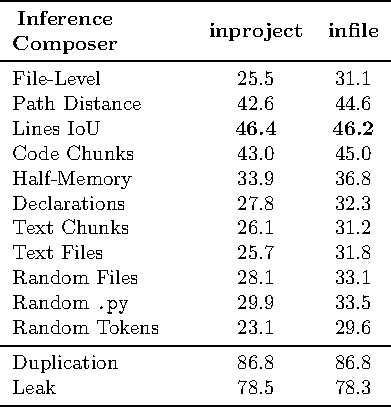
\includegraphics{tables/rq_a1.pdf}
    \caption{Exact Match scores of the DeepSeek-Coder-Base 1.3B benchmarked on the LCA}\label{tab:dseek-inference}
\end{table}

A noticeable difference is observed, allowing us to infer that the context provided to the model during inference has a significant impact on its performance. Some detailed findings are as follows:

\begin{enumerate}
\item The Lines IoU approach proposes the most effective relevance function for retrieval-augmented generation among the presented methods, demonstrating that the model can achieve the same level of \textit{inproject} performance as \textit{infile}, given the context of sufficient quality.
\item The examination of Declarations indicates that function and class declarations alone do not provide a strong foundation for in-context learning capabilities; the functional code within their bodies is more important.
\item A comparison between Random \texttt{.py} and Text Files suggests that configuration and documentation files are less important for the model than randomly selected code examples in the context. The same observation applies to code comments and documentation strings produced by Text Chunks.
\item Even randomly selected files enhance the code completion capabilities of the model.
\item Random Tokens degrade performance only slightly compared to the File-Level composer, indicating that the model is highly, though not completely, robust to the presence of noisy context.
\item The model is capable of effectively copying (Duplication) and extracting (Leak) ground truth lines from the context without requiring any additional training.
\end{enumerate}

\section{Fine-Tuning on Compositions}\label{sec:fine-tuning-on-compositions}

To estimate the impact of the context composition strategy employed during model fine-tuning, we subject the same model from the previous section to training with various composers. After fine-tuning, we benchmark the model to produce Table~\ref{tab:dseek-fine-tuning}.

\begin{table}[htbp]
    \centering
    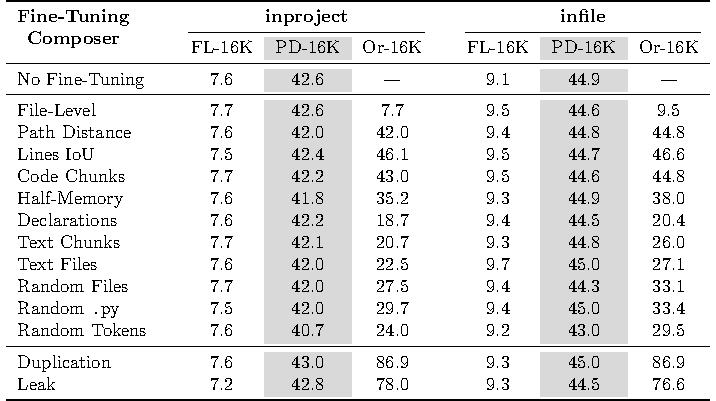
\includegraphics[width=\textwidth]{tables/rq_a2.pdf}
    \caption{Exact Match scores of DeepSeek-Coder-Base 1.3B fine-tuned with different context composition strategies. The rows indicate the composer used to obtain the model checkpoint. The columns represent different evaluation setups: PD for Path Distance, FL for File-Level, and Or for the composer used during fine-tuning. All sequences are truncated to 16K tokens. The blank cells refer to the Table~\ref{tab:dseek-inference}.}\label{tab:dseek-fine-tuning}
\end{table}

The marginal differences in metric values suggest that this particular model is sufficiently trained and is not significantly affected by subsequent fine-tuning.

One might argue that the number of training steps is insufficient. To address this concern, we monitor the learning curves during training and observe that the metric improvements are too small to justify further scaling of this experimental direction. For instance, the best linear slope, \(1.28 \times 10^{-5}\) of EM, is achieved by the Lines IoU composer during the first \(512\) iterations. Applying a linear extrapolation of this slope implies that the model would require more iterations to gain 5 EM points than permitted by the learning rate scheduler. Moreover, since the best model to approximate a learning curve is a logarithmic function, this extrapolation is extremely optimistic.  % TODO: cite scaling laws?

Additionally, we explored different setups to address the issue of the model's robustness to this type of fine-tuning. First, a different training dataset with lower data diversity was used earlier, which resulted in overfitting after the first epoch. Second, we experimented with other hyperparameter choices without success. Third, to eliminate researcher proficiency bias, the experiments were independently reproduced from scratch by another person, which is beyond the scope of this thesis.

\section{Effect of Context Extension}\label{sec:effect-of-context-extension}

\section{Influence of Composition on Context Extension}\label{sec:influence-of-composition-on-context-extension}

\section{Supplementary Results}
% TODO: gradient masking
% TODO: use term "inlier" when discussing the gradient masking impact
% TODO: highlight that we extrapolate the results of inlier gradient masking to outlier
% TODO: beyond context window
% TODO: comparison with SOTA models

\section{Limitations and Future Work}
% scale different directions, ...

% TODO: if this section is too small just wrap it as a third paragraph of the conclusion
